% article.tex, a sample LaTeX file.
% Run LaTeX on this file twice for proper section numbers.
% A '%' causes LaTeX to ignore remaining text on the line

% Use the following line for draft mode (double spaced, single column)
\documentclass[preprint,pre,floats,aps,amsmath,amssymb]{revtex4}

% Use the following line for journal mode (single spaced, double
%column)
%\documentclass[twocolumn,pre,floats,aps,amsmath,amssymb]{revtex4}
\usepackage{graphicx}
\usepackage{bm}
\usepackage{placeins}

%\renewcommand{\caption}{figure \arabic{caption}}
\usepackage[small,hang,figurename=fig.]{caption}

%\DeclareCaptionLabelFormat{UC}{\MakeUppercase{#1} #2}
%\captionsetup{labelformat=l}
\begin{document}

\title{Genesys EvE Evolutionary Processing Element Implementation}
\author{Danial Zuberi and Ethan Lyons}
\affiliation{ECE 8893: Hardware Acceleration for Machine Learning Final Project Spring 2019}
\date{May 2, 2019}

\begin{abstract}

This implementation of the EvE processing element from GeneSys [1] is part of a project for Hardware Acceleration for Machine Learning, a course at Georgia Tech. The goal of this project was to provide RTL for a processing unit that was proposed in the GeneSys paper and synthesize it to provide power and area figures.

The EvE Processing unit performs evolution on input parent genes from parent genomes. The algorithm is based on NEAT. There are four functions, Crossover, Perturbation, Delete, and Add. This PE was designed to support these four functions, as well as FIFOs to store outputs and perform some logic on inputs.

The RTL was successfully simulated, demonstrating all of the functionality for which the unit was designed. In addition, the design was successfully synthesized. A full power and area breakdown is included in the paper.

The inputs which were run through the processing elements in order to test functionality are also provided in the paper. In addition to generating simulations for one single PE, a case with multiple PEs is also demonstrated. However, this is much more difficult to trace, so most demonstrations are performed on one PE.

\end{abstract}

\maketitle

\section{Introduction}
%\label{sec:intro}

The goal of this project was to create a synthesizable RTL version of the EvE processing element. The EvE processing element is a component of Genesys, described in the paper “GeneSys: Enabling Continuous Learning through Neural Network Evolution in Hardware” written by researchers at The Georgia Institute of Technology. This GeneSys architecture is a way to implement the NEAT evolutionary algorithm. EvE is the component of the architecture that performs the evolution between generations. Parent genes are broadcast to this processing element and based on a random number generator, functions are executed on them to create a child gene. This is done over multiple processing elements in parallel to create multiple different genomes. This evolutionary algorithm shows much promise for networks that change in real time and cannot be pre-trained, as shown in the paper.


\section{Overall Design}
%\label{sec:theory}

The design of array is essentially broadcasting two 64-bit parent genes to all PEs. Then, each PE generates a random number and determines which of the functions to execute on the two genes. The steps are Crossover, Perturbation, Deletion, and Addition. When Deletion occurs, none of the other functions are executed. Each PE stores a number of output genes, which make up the next generation genome. The two best-performing genomes are used in the next generation. This implementation only includes the evolutionary PE and storing of the output genomes, not the selection of genomes. Feeding in of the parent genes is assumed to be performed by another unit.

Each of the functions that can occur during evolution is given its own module. In addition, one processing element contains three FIFOs, two for aligning parent genomes and one for storing the entire child genome.



\section{Verilog Units}

This section lists all of the verilog modules used in this implementation of the EvE processing element and describes their implementations. There is a lot of logic that goes into each stage to determine the child gene output. The overall PE is pipelined into four cycles.

\subsection{EvE}

EvE is the top module which generates an arbitrary number of PEs. The maximum acceptable number of PEs for this architecture is 255 because 0xFF is reserved for invalid. Each PE is assigned an ID, which is just a constant number used to determine the random number and identify that PE’s child genome.

\subsection{EvE\_PE}

Each PE is designed to take in two parent genes and provide anywhere between 0 and 3 output genes. Each PE generates its own child genome. The PE contains these components: the random number generator, three FIFOs, and engines for the four functions (Crossover, Perturbation, Delete, and Add). The random number generator determines which action the PE determines. It is a shift register pseudorandom number generator with an initial value based on the PE’s ID. The FIFOs are there to enable some logic. There are certain conditions in which a parent gene needs to be retained over multiple cycles, and the FIFOs enable this execution. They are driven by signals generated in the Crossover stage, which determines when to hold or use parent data, depending on node IDs. The four functions equate to a four-cycle delay. Crossover is two cycles, Perturbation is purely combinational, and Delete and Add are each one cycle.


\subsubsection{EvE\_PRNG}

EVE\_PRNG is our pseudo-random number generator. The implementation we use is a shift register format with an XOR. Each PE is designed to have a different pseudo-random number, since the initial value of the number is a concatenation of the PE’s ID with itself. Each engine is fed a different random number. This implementation uses a windowing approach, so 36 random bits are generated total.

\subsubsection{FIFO}

The FIFO is a 64-bit width, 32-bit depth FIFO. It is just a standard FIFO with reset, clock, read, write, and data inputs, with a data output. This FIFO just allows us to store parents when they aren’t used because of the node conditions. These conditions will be described in the section for the Crossover Engine, since that is the stage that implements this logic.

\subsection{EvE\_Crossover\_Engine}

The crossover engine uses windowed sections of the PRNG unit as random numbers. Based on the values of these random numbers, one of the two parent genes’ attributes are chosen. This occurs for each of the four attributes. Each attribute can either be from parent 1 or parent 2. The output of this stage is a new child gene with a new genome ID and four attributes which is some combination of the attributes of the child gene. The genome ID that is assigned to the child gene is the ID of the EvE PE. The crossover stage is pipelined into two cycles, since it is also responsible for controlling the input FIFO.

The crossover engine is responsible for determining which attributes to take from each of the parents. In this case, it is assumed that the first parent fits the neural network better than the second parent. This distinction leads to a few details in the control logic of the system. First off, in the case that the IDs of both parents match, crossover is done as normal with respect to the bias assigned in regards to how much the first parent is favored (with a low bias, more attributes from parent A will be taken). The second case is that a gene is in the first parent genome but not the second, in this case the gene is assumed to help fit the neural network better and so this gene goes straight to the perturbation engine. The third case is that a gene is in the second parent genome but not the first, in this case it is assumed this gene detrements the neural networks accuracy and a bubble is sent through the network meaning no gene is added. In both the second and third cases only one gene is being used in that cycle, for this reason it is necessary to have a FIFO which stores genes that are not used in the cycle they are fetched. This communication to read from the FIFO is also why the Crossover Engine takes two cycles.


\subsection{EvE\_Perturbation\_Engine}

The perturbation engine also uses windowed sections of the random number generator output. This implementation uses a randomly generated 3 bit number for each attribute, left-padded with zeros. This way, the maximum number that can be added to a given attribute is 7, and the minimum is 0. Four of these small perturbation numbers are generated and added to each of the gene attributes.

These perturbed attributes are multiplexed with the outputs of the crossover stage. Based on the random number generator output, either the perturbed or crossed over outputs are chosen. The output of this stage is also a child gene with the new genome ID and new attributes.

Since the Perturbation stage is very simple, it was designed to be purely combinational. It is not pipelined, but can be if it is determined that it would benefit performance.


\subsection{EvE\_Delete\_Engine}

The Deletion engine also uses the random number generator to decide if a node will be deleted. There is a counter, since there is a limit to the number of nodes that can be deleted. If the probability is met and the counter is not at the maximum value, the node is deleted. Otherwise, the gene passes through. The one exception is when there is a dangling connection. Dangling connections are handled by a unit called Deleted\_Nodes, which keeps track of nodes that have been deleted such as to identify dangling connections.

\subsubsection{Deleted\_Nodes}

The Deleted Nodes unit keeps track of deleted nodes until it is full, at which point no more nodes can be deleted. The main purpose of this unit is to look at the input gene and check if it is a dangling connection. If one of the two nodes on the connection matches a stored node ID, it is a dangling connection and must also be deleted. It essentially contains a number of comparators connected to each stored gene entry, a reset switch, and some storage. The output is a signal called “match”, which is always asserted when either of the two IDs of a connection are found in the storage.

\subsection{EvE\_Add\_Gene\_Engine}

This is a variable width and variable depth FIFO which will be responsible for holding all of the valid child genes. Each PE will have one of these buffers and it will be responsible for storing the whole neural network. After evaluating all of the child genes, the two best genomes can be picked and these child genes can just be released from the FIFO, reordered in the split and merge units, and then they will become the parents for the next generation. All of the genomes which will not become the next set of parent can then just be flushed out of the FIFO.
\newline \indent
The key component of this FIFO is that it is able to take in three inputs at the same time and update the writing pointers accordingly. Specifically, it is able to add 0, 1, 2, or 3 child genes to the FIFO at the same time. This corresponds to the potential number of genes that will be created by the add gene engine. It is useful that it is a FIFO as the child node genes will enter into the FIFO in order and therefore will not have to be reordered. Additionally, the child genes which were not generated in the add gene engine will also be in order. Therefore, the benefit of making this structure a FIFO is that the only things which will need to be reordered for the next generation are the new connections which are added within the add gene engine.

\subsubsection{Triple-Ported Buffer}

This is a variable width and variable depth FIFO which will be responsible for holding all of the valid child genes. Each PE will have one of these buffers and it will be responsible for storing the whole neural network. After evaluating all of the child genes, the two best genomes can be picked and these child genes can just be released from the FIFO, reordered in the split and merge units, and then they will become the parents for the next generation. All of the genomes which will not become the next set of parent can then just be flushed out of the FIFO.

The key component of this FIFO is that it is able to take in three inputs at the same time and update the writing pointers accordingly. Specifically, it is able to add 0, 1, 2, or 3 child genes to the FIFO at the same time. This corresponds to the potential number of genes that will be created by the add gene engine. It is useful that it is a FIFO as the child node genes will enter into the FIFO in order and therefore will not have to be reordered. Additionally, the child genes which were not generated in the add gene engine will also be in order. Therefore, the benefit of making this structure a FIFO is that the only things which will need to be reordered for the next generation are the new connections which are added within the add gene engine.


\section{Results}
%\label{sec:analysis}
The implementation was successful. Both simulation and synthesis results are presented in this section.
\subsection{Simulations}
The simulation results follow. Various functions of the PE are presented and described. Values that are not relevant to that function have been blacked out for clarity.

\subsubsection{Crossover Bubble}

\begin{figure}[htb!]
	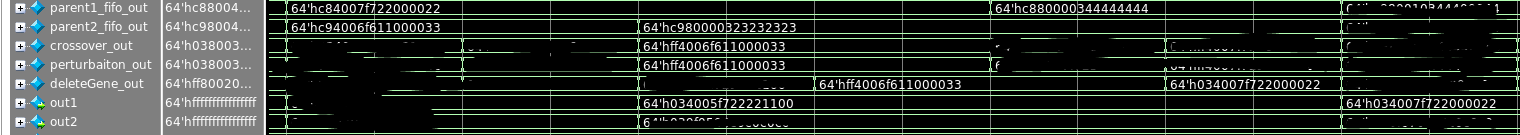
\includegraphics[width=\textwidth]{Crossover_Bubble}
	\caption{Crossover Bubble Functionality}
\end{figure}
\FloatBarrier
Above is an example of the case in which the second parent has a gene which the first parent does not have. As can be seen, once this gene leaves the crossover engine it has been turned into an invalid gene (a bubble) which is denoted by setting the first two bytes, which represent the genome ID, to 0xFF.

\newpage
\subsubsection{Delete Node}

\begin{figure}[htb!]
	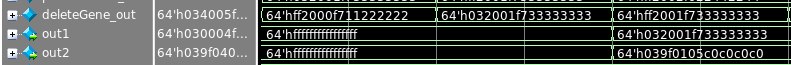
\includegraphics[width=\textwidth]{DeleteNode}
	\caption{Delete Node Functionality}
\end{figure}
\FloatBarrier
This is an example of a node which has been deleted (with ID 0x00). It can be seen that this node was never sent as one of the outputs due to the fact that it was deleted.

\subsubsection{Delete Dangling}

\begin{figure}[htb!]
	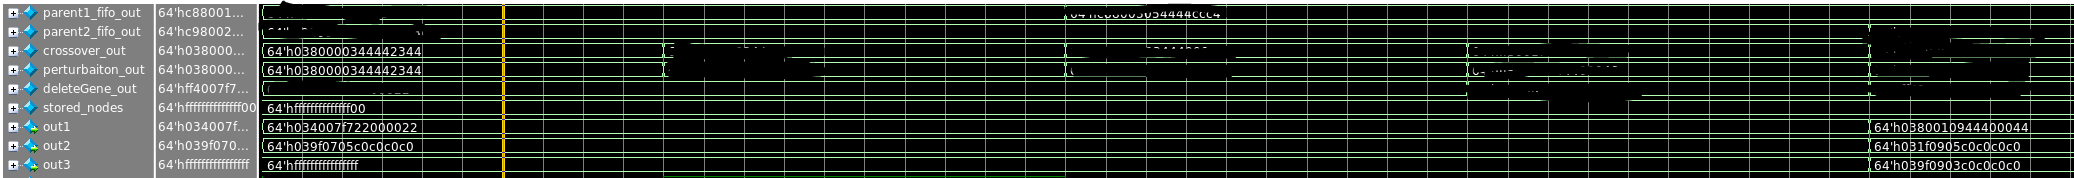
\includegraphics[width=\textwidth]{DeleteDangling}
	\caption{Delete Dangling Functionality}
\end{figure}
\FloatBarrier
Going off of the previous example, it can be seen that the node with ID 0x00 was deleted and therefore all dangling connections need to be deleted. It can be seen in this waveform that a connection from node 0 to node 3 made its way through the perturbation engine but then gets deleted in the delete gene engine and never gets outputted from the pipeline.

\subsubsection{Add Connection}

\begin{figure}[htb!]
	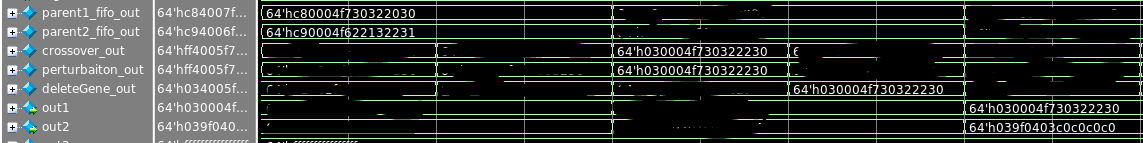
\includegraphics[width=\textwidth]{AddConnection}
	\caption{Add Conection Functionality}
\end{figure}
\FloatBarrier
This shows a connection being added when nodes are streaming. It can be seen that the new connection attributes are all set to 0xC0 (the default value)

\newpage
\subsubsection{Add Node}

\begin{figure}[htb!]
	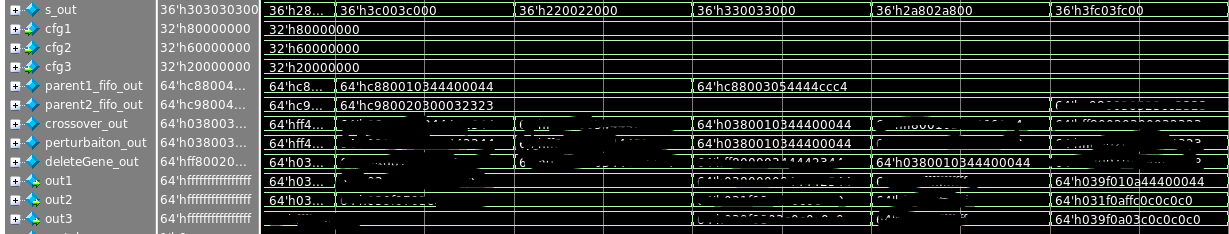
\includegraphics[width=\textwidth]{AddNode+ParentB_Stall}
	\caption{Add Node Functionality}
\end{figure}
\FloatBarrier
This shows the addition of a node when streaming connections. It can be seen that the initial connection from node 1 to 3 is split and a new node is added (node A) as well as a connection from node 1 to node A and a connection from node A to node 3. Additionally the stalling of reading inputs can be seen in the case of parent 2.

\subsubsection{Outputs Stored}

\begin{figure}[htb!]
	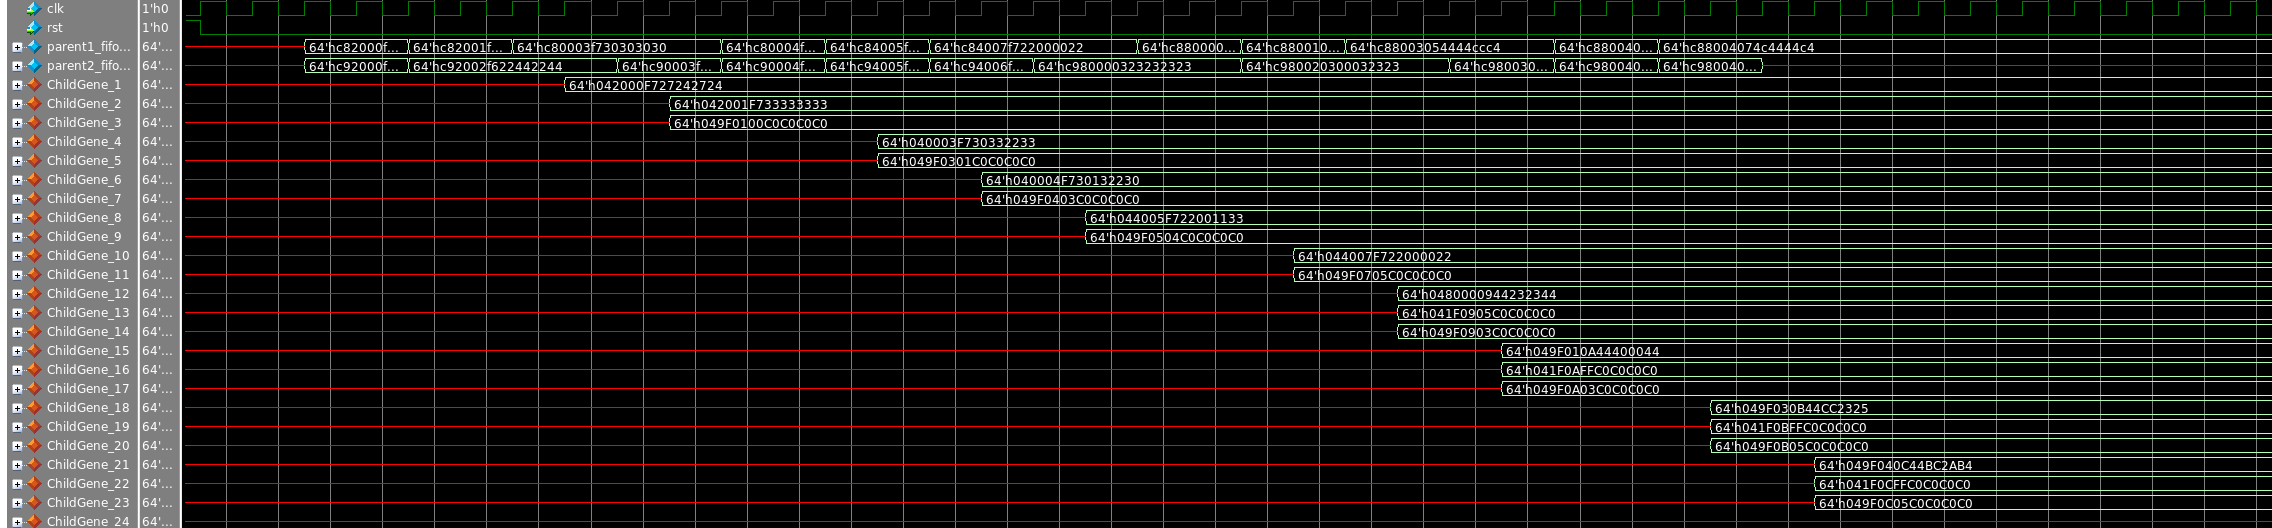
\includegraphics[width=\textwidth]{OutputsStored}
	\caption{Outputs Stored Functionality}
\end{figure}
\FloatBarrier
This shows the storage of all of the child genes which are created within one PE in the output FIFO. All these valid genes will be used to test the network and then will easily be able to become parents in the next generation if they are selected.

\newpage
\subsubsection{Multiple PEs}

\begin{figure}[htb!]
	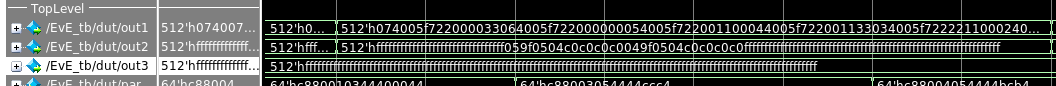
\includegraphics[width=\textwidth]{Multiple_PE}
	\caption{Multiple PE Functionality}
\end{figure}
\FloatBarrier
This figure shows the functioning of an array of PEs all running at the same time. It can be seen that they produce different output genes which occurs due to the different random number generators. This is good as it is beneficial to have lots of diversity when performing genetic algorithms.

\subsubsection{Test cases used}
\begin {figure} [h!]
	\begin{center}
		\begin{tabular}{|c|c|c|c|}
			\hline
			Parent A& Description & Parent B & Description \\ \hline
			C82000F722222222& Node 0x0 &C92000F611331133  & Node 0x0 \\ \hline
			C82001F733333333& Node 0x1 &C92002F622442244 & Node 0x2 \\ \hline
			C80003F730303030& Node 0x3 &C90003F622332233 & Node 0x3 \\ \hline
			C80004F730322030& Node 0x4 &C90004F622132231 & Node 0x4 \\ \hline
			C84005F722220000&  Node 0x5&C94005F600001133 & Node 0x5 \\ \hline
			C84007F722000022& Node 0x7&C94006F611000033 & Node 0x6 \\ \hline
			C880000344444444& Connection 0x0  $\rightarrow$  0x3&C980000323232323 & Connection 0x0  $\rightarrow$  0x3 \\ \hline
			C880010344400044& Connection 0x1  $\rightarrow$  0x3&C980020300032323 & Connection 0x2  $\rightarrow$  0x3 \\ \hline
			C88003054444CCC4& Connection 0x3  $\rightarrow$  0x5&C980030523CC2323 & Connection 0x3  $\rightarrow$  0x5 \\ \hline
			C88004054444BCB4& Connection 0x4  $\rightarrow$  0x5&C980040523BC2626 & Connection 0x4  $\rightarrow$  0x5 \\ \hline
			C88004074C4444C4& Connection 0x4  $\rightarrow$  0x7&C98004062B2323B3 & Connection 0x4  $\rightarrow$  0x6 \\ \hline
		\end{tabular}
	\end{center}
	\caption{Table of parent genes used to test functionality}
\end{figure}
\FloatBarrier
The table above lists all parent genes that were used to test the functionality of our implementation of the EvE PE.

\subsection{Synthesis}
\begin{figure}[h!]
	\begin{center}
		\begin{tabular}{|c|c|c|}
			\hline
			Source & Power (mW) & Area($\mu m^2$)  \\ \hline
			Total & 13.673 & 14710.95\\ \hline
			Output FIFO & 3.281 & 4266.3935\\ \hline
			2x Input FIFO & 4.439 & 4510.5806\\ \hline
			Crossover & 0.342 & 325.7795\\ \hline
			Perturbation & 0.143 & 165.5439\\ \hline
			Delete & 0.360 & 440.0579\\ \hline
			Add & 0.496 & 411.845\\ \hline
			PRNG & 0.177 & 80.1669\\ \hline

		\end{tabular}
	\end{center}
	\caption{Area and Power Breakdown}

\end{figure}
\FloatBarrier
A single EvE PE was synthesized in Synopsys to obtain Area and Power figures. Above is a table containing the breakdown of the area and power numbers. It is clear that the FIFOs take up a significant portion of both the area and power, but that is as expected.

\section{Conclusion}
The results show the implementation of the PE of an accelerator aimed at accelerating neural networks which are generated using genetic algorithms, similarly to what is done in the GeneSys paper. The accelerator has a throughput of one parent gene per cycle and a latency of four cycles. Additionally, an array of PEs was arranged and evaluated to represent the population that is generated for a given generation. Future work would be to implement the gene split and gene merge blocks so that child genes can be reordered so that they can be successfully processed in the next generation. In addition, adding ADAM is of obvious importance since we currently have no way to evaluate a genome in order to  choose the parents for the next generation.


\section{References}
[1] GeneSys: Enabling Continuous Learning through Neural Network Evolution in Hardware, Ananda Samajdar, Parth Mannan, Kartikay Garg, and Tushar Krishna In Proc of 51st Annual IEEE/ACM International Symposium on Microarchitecture (MICRO), Oct 2018
%\label{sec:References}
\end{document}
